%Modified from a template provided by Jennifer Pan, August 2011

\documentclass[10pt,letter]{article}
	% basic article document class
	% use percent signs to make comments to yourself -- they will not show up.
\usepackage{pdfsync}
\usepackage{amsmath}
\usepackage{amssymb}
\usepackage{amsthm}
\usepackage[makeroom]{cancel}
	% packages that allow mathematical formatting

\usepackage{graphicx}
	% package that allows you to include graphics
\graphicspath{ {./images/} }


\usepackage{subcaption}

\usepackage{setspace}
	% package that allows you to change spacing

\onehalfspacing
	% text become 1.5 spaced

\usepackage{fullpage}
% package that specifies normal margins

\usepackage[parfill]{parskip}

\newtheorem*{thm}{Theorem}
\newtheorem{nthm}{Theorem}
\newtheorem{lem}{Lemma}

\begin{document}
	% line of code telling latex that your document is beginning

\title{Problem Set 5}

\author{Katherine Cheng, Richard Davis, Marty Keil}

% \date{Friday April 10, 2015}
	% Note: when you omit this command, the current date is automatically included
 
\maketitle 
	% tells latex to follow your header (e.g., title, author) commands.

\section*{Problem One} Richard Davis submitted these.

\section*{Problem Two} Marty Keil submitted these.

\section*{Problem Three} 

\paragraph{iv.} 
epsilon | a | ( b | aa | ab(a|b) ) (a|b)*

\section*{Problem Four: Powerset of $\Sigma^*$}
If $\Sigma$ is an alphabet, then $\Sigma^*$ is the set of all strings composed from letters in $\Sigma$. The powerset of $\Sigma^*$ is the set of all $\Sigma^*$'s subsets. In other words, the powerset is the set of all possible languages in the alphabet $\Sigma$. 

\section*{Problem Five: Cardinalities and Concatenations}
Prove or disprove: if $L$ is a language and $k \ge 1$, then $|L^k| = |L|^k$. (As a special case, the language $L^0$ is defined to be $\{\varepsilon\}$.) 

This can be proved with a combinatorics argument. There are $|L|$ choices for the first string, $|L|$ choices for the second string, and so on. This means there are $|L|^k$ ways to make a concatenated string. 

\section*{Problem Six: Finite and Cofinite Languages}

\paragraph{i)} I think this can be solved using induction. Take any finite language. Treat it like two concatenated languages. Break these apart and prove (using complete induction) that they are both regular. Their concatenation is also regular. See slide 6 of Small15.pdf.

\paragraph{ii)} Remember that to complement a regular language we represent it as a DFA and flip all the states. This means we can start with a cofinite language, represent it as a DFA, then flip the states and still have a regular language. Then we use the proof from part i) to finish the proof.

\section*{Problem Seven: State Elimination}

\paragraph{i.} After bypassing states $q1$ and $q2$ we get the following DFA:\\

\begin{figure}[h]
\centering
  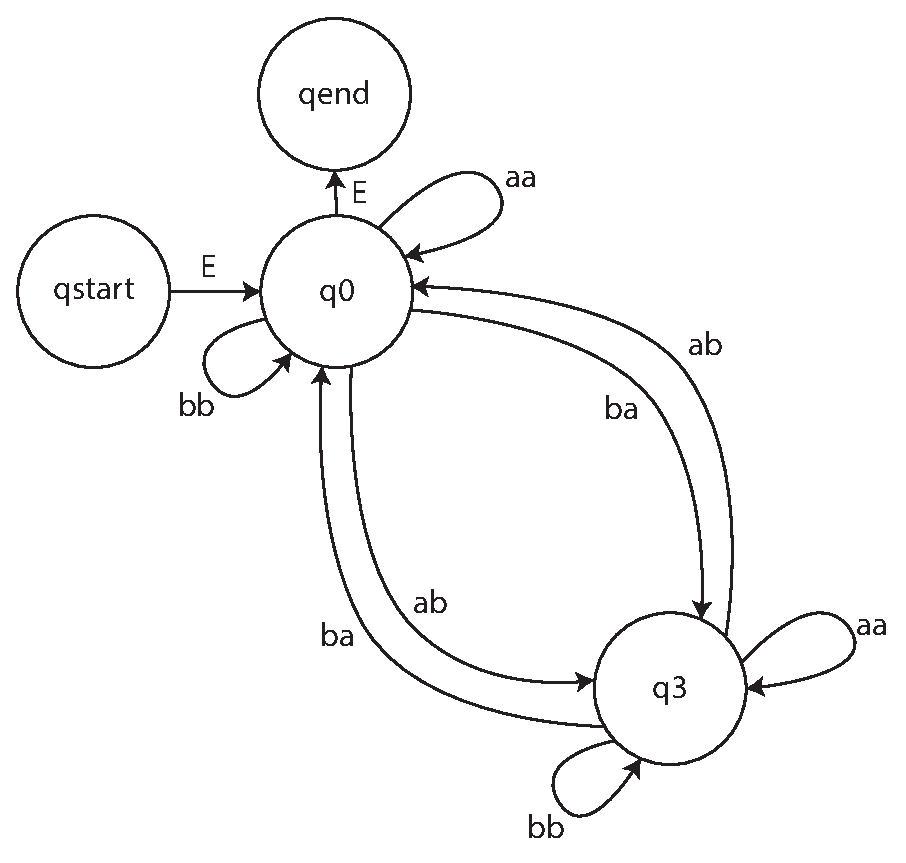
\includegraphics[width=0.45\linewidth]{7i.eps}
  \caption{DFA after bypassing q1 and q2}
  \label{fig:7i}
\end{figure}

\paragraph{ii.} After everything I got $( (aa|bb) | (ab|ba) (aa|bb)^* (ab|ba))^*$.

\section*{Problem Eight: Derivatives of Regular Languages}

\paragraph{i)} Pick some arbitrary character $k$ that we are taking the derivative of. Take the first transition from the start state using character $k$. Make this the new start state. If there is no transition out of the start state on character $k$, delete the entire DFA.

\Paragraph{ii)} 

\section*{Problem Nine: Why the Extra State?} 
One of the languages that this does not work for is defined by the regular expression \texttt{a*b}. This can be represented by the NFA that looks like this:

\begin{figure}[h]
\centering
  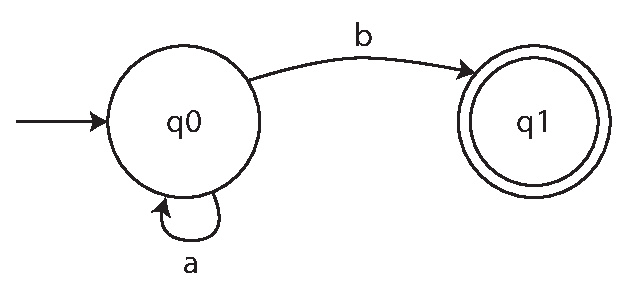
\includegraphics[width=0.45\linewidth]{9i.eps}
  \caption{NFA for \texttt{a*b}}
  \label{fig:9i}
\end{figure}

If we try to make an epsilon transition back to the start state and make that an accepting state, we end up with the following NFA.

\begin{figure}[h]
\centering
  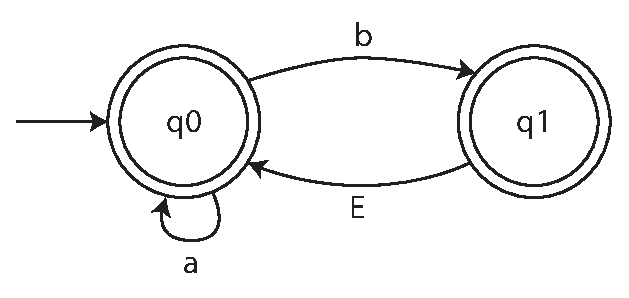
\includegraphics[width=0.45\linewidth]{9ii.eps}
  \caption{Wrong NFA for \texttt{a*b}}
  \label{fig:9ii}
\end{figure}

This ends up accepting, for example, the string ``a,'' which is not a part of the language.

% \Section*{Appendix: Referencing Equations}
% \begin{equation} \label{eq:divbyzero}
%   \frac {1} {0}
% \end{equation}

% This references \ref{eq:divbyzero}.

% \section*{Appendix: Figures in Text}
% Below are two different ways of placing figures side by side in text. The first method creates two sub-figures within a single figure. The second method creates two separate figures.

% \begin{figure}
% \centering
% \begin{minipage}{.5\textwidth}
%   \centering
%   \includegraphics[width=.8\linewidth]{hw3_8_1.eps}
%   \captionof{figure}{A figure}
%   \label{fig:q8_test1}
% \end{minipage}%
% \begin{minipage}{.5\textwidth}
%   \centering
%   \includegraphics[width=.8\linewidth]{hw3_8_1.eps}
%   \captionof{figure}{Another figure}
%   \label{fig:q8_test2}
% \end{minipage}
% \end{figure}


% \begin{figure}[h]
%   \centering

%   \begin{subfigure}[b]{0.3\textwidth}
%     \includegraphics[width=\textwidth]{hw3_8_1.eps}
%     \caption{A cycle with length $k+1$}
%     \label{fig:q8_cycle:a}
%   \end{subfigure}% 
%   \qquad
%   \begin{subfigure}[b]{0.3\textwidth}
%     \includegraphics[width=\textwidth]{hw3_8_1.eps}
%     \caption{A cycle with length $k+1$}
%     \label{fig:q8_cycle:b}
%   \end{subfigure}%  

%   \caption{Placeholder}
%   \label{fig:q8}
% \end{figure}

\end{document}
	% line of code telling latex that your document is ending. If you leave this out, you'll get an error

%%% Local Variables:
%%% mode: latex
%%% TeX-master: t
%%% End:
